\documentclass[dvipdfmx]{jarticle}
\usepackage{graphicx}
\usepackage[top=30truemm,bottom=30truemm,left=25truemm,right=25truemm]{geometry}
\usepackage{listings,jvlisting}
\usepackage{url}

\lstset{
  basicstyle={\ttfamily},
  identifierstyle={\small},
  commentstyle={\smallitshape},
  keywordstyle={\small\bfseries},
  ndkeywordstyle={\small},
  stringstyle={\small\ttfamily},
  frame={tb},
  breaklines=true,
  columns=[l]{fullflexible},
  numbers=left,
  xrightmargin=0zw,
  xleftmargin=3zw,
  numberstyle={\scriptsize},
  stepnumber=1,
  numbersep=1zw,
  lineskip=-0.5ex
}

\begin{document}
\begin{titlepage}
    \begin{center}
        {\huge データベースSQL演習課題}
        \vspace{180pt}\\
        \begin{tabular}{rl}
            氏名 & 山久保孝亮\\
            所属 & 大阪大学基礎工学部情報科学科ソフトウェア科学コース\\
            メールアドレス & u327468b@ecs.osaka-u.ac.jp\\
            学籍番号 & 09B22084\\
            提出日 & \today\\
        \end{tabular}
    \end{center}
\end{titlepage}
\section{課題1}
\subsection{課題内容}
学生名'Aomori'が履修している科目の授業担当の教員の教員名を求めよ.
\subsection{SQL文}

\subsection{解法}
課題1で最終的に出力する内容は教授名であるため,SELECT文にはlecturer.nameとした.\\
履修しているかどうかの情報はregistration,教授がどの科目を担当しているかはlectured\_by,学生名が'Aomori'かどうかはstudentテーブルを参照する必要がある.
したがってlecturerと上記3つのテーブルを結合することにより学生名を参照すれば担当している教授名を参照できるようになる.
また,DISTINCTを入れた理由としては,'Aomori'という学生が同じ教授の授業を複数履修しており問い合わせの結果に同じ教授名が二回以上出力されないようにするためである.
\subsection{問い合わせの結果}
\begin{figure}[h]
    \centering
    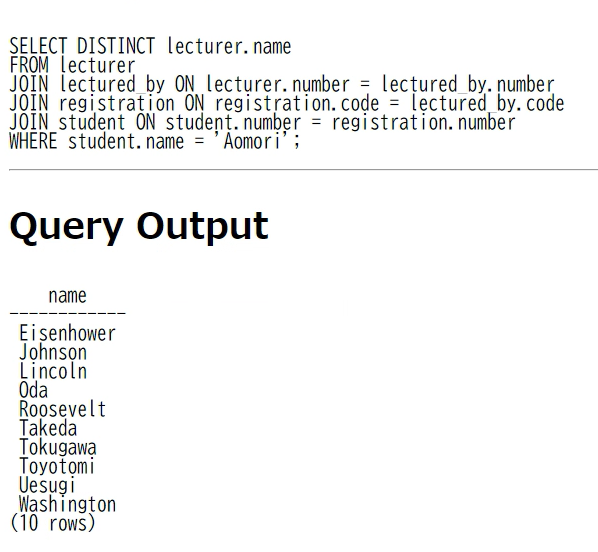
\includegraphics[width = 10cm]{1.png}
    \caption{問い合わせの結果}
\end{figure}
\section{課題2}
\subsection{課題内容}
履修者が最も少ない科目の科目番号と履修者数を求めよ.
\subsection{SQL文}
\subsection{解法}
\subsection{問い合わせの結果}
\section{課題3}
\subsection{課題内容}
科目ごとに成績の最も高い学生の成績と学生名を科目番号とともに求めよ.
\subsection{SQL文}
\subsection{解法}
\subsection{問い合わせの結果}
\section{課題4}
\subsection{課題内容}
必修の科目をすべて履修している学生の学籍番号を求めよ.
\subsection{SQL文}
\subsection{解法}
今回の課題は以下の流れで処理を進めた.
\begin{enumerate}
    \item 全生徒の内,一人に着目する.
    \item 全講義の内,一つの必修の講義のみに着目する.
    \item 着目している生徒が,着目している必修の講義を履修しているかどうかを確認する.
    \item 2,3を全ての必修の講義に対して行う.
    \item 1,2,3,4を全生徒に対して行う.
\end{enumerate}
また,今回の課題ではNOT EXISTを用いた.NOT EXISTは()内でのSELECT文の結果一つも存在しなければTRUEを返すというものである.
今回は必修の科目をすべて履修している学生を考えているが,NOT EXISTを二回用いることでこれを実現した.
一つ目のNOT EXISTでは「必修の講義をすべて履修している」ことを「履修していない必修の講義が存在しない」と見なして利用した.
二つ目のNOT EXISTでは「」
\subsection{問い合わせの結果}
\end{document}